\documentclass{article}
\usepackage{graphicx} % Required for inserting images
\usepackage[margin=1in,footskip=0.25in]{geometry}
\usepackage{stmaryrd}
 \usepackage{amsmath}
\usepackage{tikz}
\usetikzlibrary{matrix, positioning}
\title{WorkMeetings}
\date{January 2024}
\usepackage{fontawesome5}
\usepackage{hyperref}
\definecolor{BleuLMS}{RGB}{1, 66, 106}
\definecolor{GreenLMS}{RGB}{0,103,127} 
\hypersetup{
    colorlinks=true,
    citecolor=BleuLMS,
    linkcolor=BleuLMS,
    filecolor=BleuLMS,      
    urlcolor=GreenLMS,
    pdftitle={Overleaf Example},
    pdfpagemode=FullScreen,
    }
\begin{document}

\maketitle


\section{Progress report}
At the point of the meeting, we both have an implementation of a HiDeNN for solving the clamped 1D bar problem. Both of our implementations work when finding nodal coordinates onto a fixed mesh (i.e., solving the finite element problem by training the Neural Network and tuning the weight of the last hidden layer). However, there are still some issues when training the coordinates values of the mesh nodes. Indeed, the gradients are not correctly populated in deeper layers and the gradient of the loss w.r.t the coordinates only accounts for the operations occurring in the first layer. 

A manner to pass trainable arguments into forward functions and still populate their gradients for the downstream operations is yet to be found. A \href{https://discuss.pytorch.org/t/reusing-altered-parameters-in-more-than-one-layer/158106/2}{promising lead} was found by Katka at the end of the day, but it remains to be tested.

We have two different implementations. 
\begin{itemize}
    \item[\faCodeBranch] \textbf{Option a)} only relies on two ``global'' NN that are latter combined. 
    \item[\faCodeBranch] \textbf{Option b)} is more fragmented and is built on sub-neural networks that correspond to the elementary blocks described in \cite{zhang_hierarchical_2021}.
\end{itemize}

\section{Required tools in the future}

For future application, several implementations are required. 
\begin{itemize}
    \item[\faCogs] 1D bar elements 
    \begin{itemize}
            \item[\faChevronRight] Linear
        \item[\faChevronRight] Quadratic
    \end{itemize}
    \item[\faCogs] 2D triangles
    \begin{itemize}
        \item[\faChevronRight] Linear (T3)
        \item[\faChevronRight] Quadratic (T6)
    \end{itemize}
    \item[\faCogs] 2D quadrangles
    \begin{itemize}
        \item[\faChevronRight] Linear
        \item[\faChevronRight] Quadratic
    \end{itemize}
\end{itemize}

In order to use the Gauss quadrature, it is necessary to implement the reference element for each of these elements and to map the reference elements to the real elements. The reference elements are non-trainable blocks that are hard coded, and the mapping (relying on the actual nodal coordinates) is tuned through the training process. The mapping can remain linear even for quadratic shape functions for now.


\section{Spatial parameters}
An essential aspect for the future relies on non-uniform parameters across the considered geometry. Making patient-specific models also means adapting those parameter fields to each new patient. In order for the Neural Network (NN) to be usable for a new spatial distribution of parameters $\mu\left(x\right)$ (i.e., a new patient), the spatial distribution, somehow must be part of the input of the neural network (as opposed to solely inputting the value of the parameter at the coordinate we evaluate the NN).
% \subsection{Parameter field representation}
In order to account for the global aspect of the spatial distribution without relying on an enormous number of parameters, an idea is to project the parameter field onto a spatial basis of a reasonable size. The Parameter field would then read 
\begin{equation}
    \mu\left(x\right) = \sum_{i=1}^{n_p}\mu_i f_i\left(x\right), 
    \label{eq:Projection_parameterField}
\end{equation}
with $\left\{f_i\right\}_{i \ in \llbracket 1,n_p \rrbracket}$ a spatial basis composed of global functions. A naive (and inefficient) idea for the basis basis would be to use discontinuous Galerkin functions to span the parameter space. Later, a more suitable basis could instead be obtained using several training data (actual parameter fields). The patient-specific input values $\left\{\mu_i\right\}_{i \ in \llbracket 1,n_p \rrbracket}$ would then correspond to the coordinates of the projection of the new patient parameter field $\mu(x)$ onto the previously computed basis.

% \begin{figure}
%     \centering
%     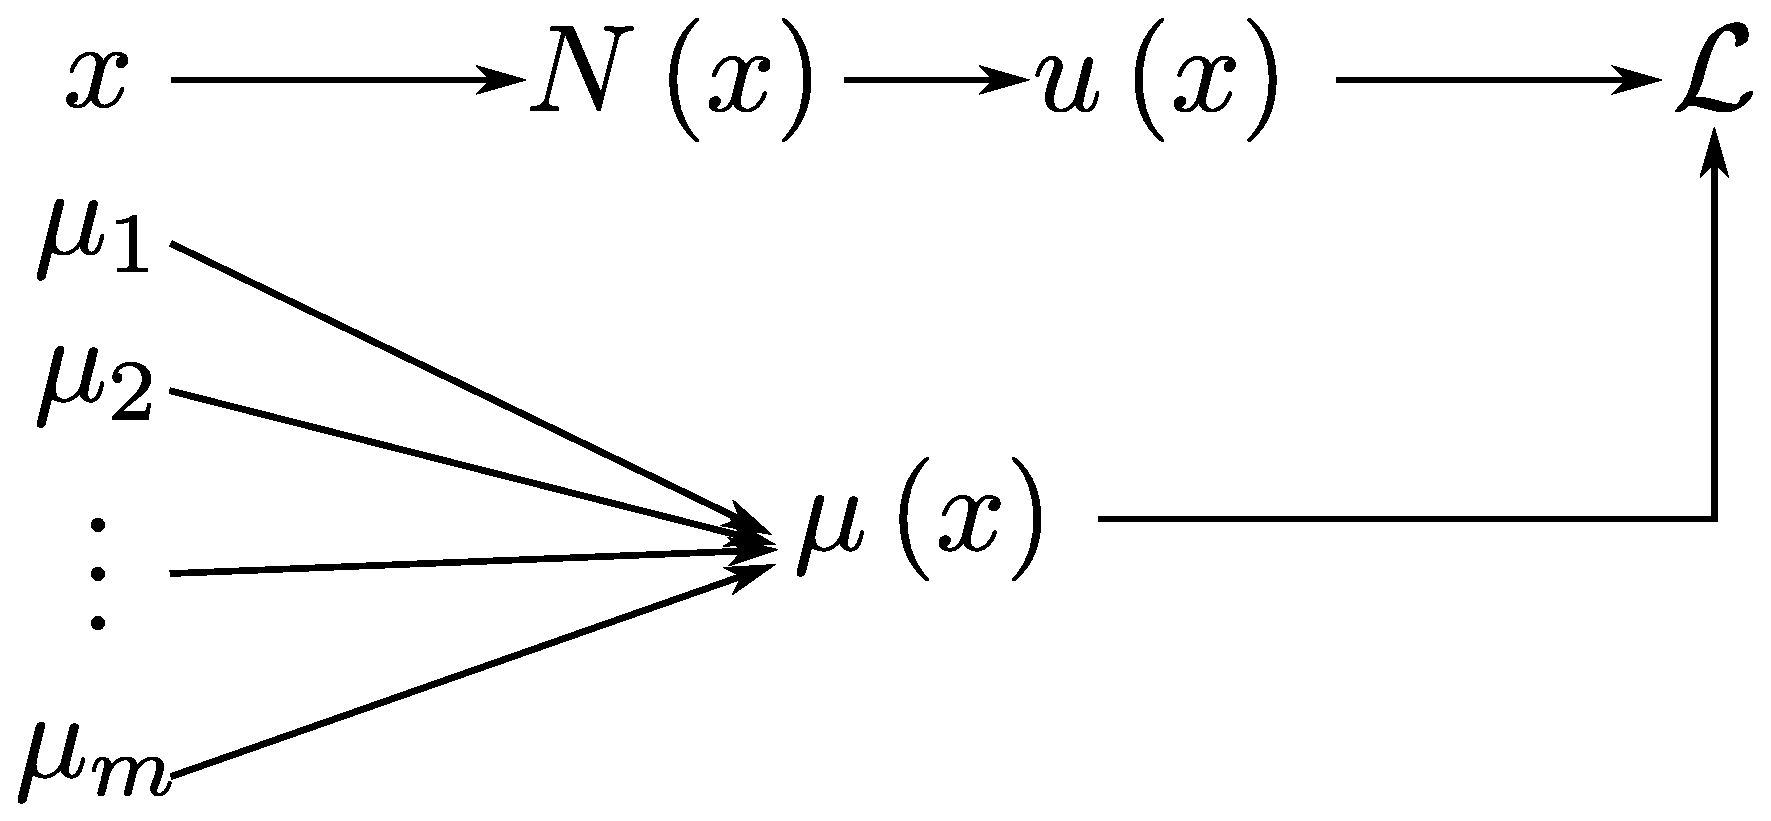
\includegraphics[width = 0.7\linewidth]{Figures/SpatialVariability_Parameters.eps}
%     \caption{Architecture of the HiDeNN parametrised with spatial parameter fields}
%     \label{SpatialVariability}
% \end{figure}

\begin{figure}[h]
    \centering
    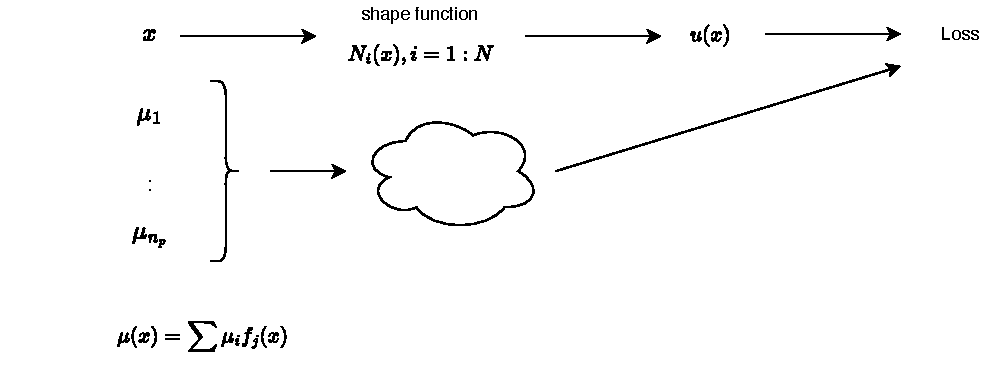
\includegraphics[width = 0.8\linewidth]{Figures/Diagram_1.pdf}
    \caption{Architecture of the HiDeNN parametrised with spatial parameter fields}
    \label{SpatialVariability}
\end{figure}

\section{Integral formulation of loss vs. Mixed formulation}

For the 1D test problem:
\begin{align*}
    \frac{\mathrm{d}}{\mathrm{d}x}\left( AE \frac{\mathrm{d}u}{\mathrm{d}x}\right) + b(x) = 0 \quad x\in [0,10]
\end{align*}
we use (i) integral loss function approach, (ii) mixed formulation approach. 

In (i) we perform forward pass of NN to get $u(x)$ for all training points $x$, then evaluate loss, compute gradient and update NN weights. To evaluate the loss, we use $\frac{\mathrm{d}u}{\mathrm{d}x}$ obtained by autograd -- linear shape functions are sufficient.

In (ii), we define two NNs: one for prediction of $u(x)$ and one for prediction of $s(x) = E\frac{\mathrm{d}u}{\mathrm{d}x}$. Loss function consists of two terms:
\begin{align*}
    \mathrm{Loss}(x) = \| \frac{\mathrm{d}}{\mathrm{d}x}\left( As(x)\right) + b(x)\|^2 + \| s(x) - E\frac{\mathrm{d}u}{\mathrm{d}x}\|^2
\end{align*}
The training points are processed individually or in batches  -- weights are be updated after evaluation of each points / batch. We use NN with quadratic shape functions for predictions of $u$ and NN with linear shape function for predictions of $s$.
\begin{figure}[h!]
    \centering
    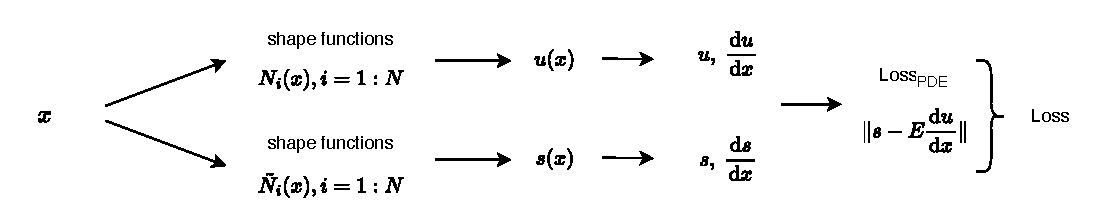
\includegraphics[width = 0.8\linewidth]{Figures/Diagram_2.pdf}
    \caption{The two NNs used for the mixed formulation.}
\end{figure}


\bibliographystyle{apalike} % We choose the "plain" reference style
\bibliography{biblio} % Entries are in the refs.bib file
\end{document}
